\chapter{AXI4-Lite interface}
\section{Structure}
The AXI4-Lite interface for this core acts as a slave to the AXI bus. It only supports the AXI-Lite procotol since there
is no ID reflection of the data transfer and only a 32-bit wide bus is supported. The AXI4-Lite IPcore block contains the
exponentiation core and a control register for the core its control inputs and outputs.

\section{Parameters}
This section describes the parameters used to configure the core, only the relevant parameters are discussed. AXI
specific parameters are left to the user to configure. The IP core specific parameters and their respective use are
listed in the table below.
\begin{center}
	\begin{tabular}{|l|p{6.5cm}|c|l|}
		\hline
		\rowcolor{Gray}
		\textbf{Name} & \textbf{Description} & \textbf{VHDL Type} &\textbf{Default Value} \bigstrut\\
		\hline
		\multicolumn{4}{|l|}{\textit{\textbf{Memory configuration}}} \\		
		\hline
		\verb|C_FIFO_DEPTH| & depth of the generic FIFO, only applicable if \verb|C_MEM_STYLE| = \verb|"generic"| or \verb|"asym"|  & integer & 32 \bigstrut\\
		\hline
		\verb|C_MEM_STYLE| & the memory structure to use for the RAM, choice between 3 options: & string & \verb|"generic"| \bigstrut\\
							& \verb|"xil_prim"| : use xilinx primitives & & \\
      						& \verb|"generic"| : use general 32-bit RAMs & & \\
      						& \verb|"asym"| : use asymmetric RAMs & & \\
      						& (For more information see \ref{subsec:RAM_and_FIFO}) & & \bigstrut[b] \\
		\hline
		\verb|C_FPGA_MAN| & device manufacturer: & string & \verb|"xilinx"| \\
						& \verb|"xilinx"| or \verb|"altera"| &  &  \bigstrut\\
		\hline
		\verb|C_BASEADDR| & base address for the IP core's memory space & std\_logic\_vector & X"FFFFFFFF" \bigstrut\\
		\hline
		\verb|C_HIGHADDR| & high address for the IP core's memory space & std\_logic\_vector & X"00000000" \bigstrut\\
		\hline
		\multicolumn{4}{|l|}{\textit{\textbf{Multiplier configuration}}} \\
		\hline
		\verb|C_NR_BITS_TOTAL| & total width of the multiplier in bits & integer & 1536\bigstrut\\
		\hline
		\verb|C_NR_STAGES_TOTAL| & total number of stages in the pipeline & integer & 96\bigstrut\\
		\hline
		\verb|C_NR_STAGES_LOW| & number of lower stages in the pipeline, defines the bit-width of the lower pipeline part & integer & 32 \bigstrut\\
		\hline
		\verb|C_SPLIT_PIPELINE| & option to split the pipeline in 2 parts & boolean & true \bigstrut\\
		\hline
	\end{tabular}%
\end{center}
%\newline 
\newpage
The IP core's memory space is organised in a fixed structure as show in Figure~\ref{AXImemstructure}. Only the upper 17
bits (31:15) of the base address can be chosen freely, the lower bits must be 0. So the \verb|C_BASEADDR| parameter must end
in 0xXXXX0000 or 0xXXXX8000 in hexadecimal representation. The core's memory space must have a minimum width of 28K byte for 
all registers to be accessible.
\begin{figure}[H]	
\centering
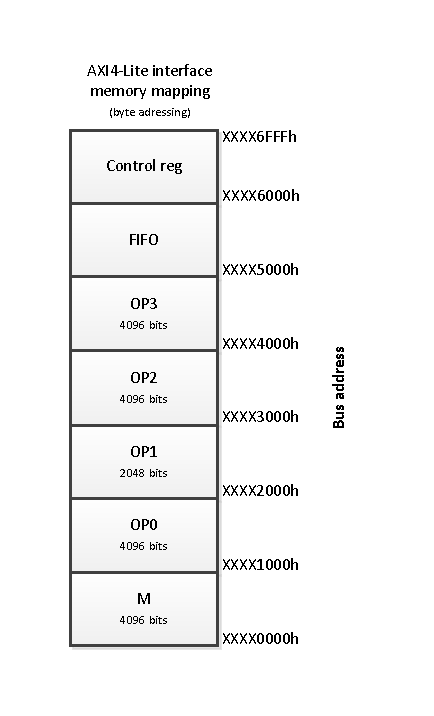
\includegraphics[trim=1.2cm 1.2cm 1.2cm 1.2cm, width=5cm]{pictures/axi_mem.pdf}
\caption{AXI4-Lite IP core memory structure}
\label{AXImemstructure}
\end{figure}

There are 4 parameters to configure the multiplier. These values define the width of the multiplier operands and the
number of pipeline stages. If \verb|C_SPLIT_PIPELINE| is false, only operands with a width of\\\verb|C_NR_BITS_TOTAL| are
valid. Else if \verb|C_SPLIT_PIPELINE| is true, 3 operand widths can be supported:
\begin{itemize}
  \item the length of the full pipeline ($C\_NR\_BITS\_TOTAL$)
  \item the length of the lower pipeline ($\frac{C\_NR\_BITS\_TOTAL}{C\_NR\_STAGES\_TOTAL} \cdot C\_NR\_STAGES\_LOW $)
  \item the length of the higher pipeline ($\frac{C\_NR\_BITS\_TOTAL}{C\_NR\_STAGES\_TOTAL} \cdot (C\_NR\_STAGES\_TOTAL - C\_NR\_STAGES\_LOW$)
\end{itemize}

\section{IO ports}
\begin{tabular}{|l|c|c|l|}
	\hline
	\rowcolor{Gray}
	\textbf{Port} & \textbf{Width} & \textbf{Direction} & \textbf{Description} \\
	\hline
	\multicolumn{4}{|l|}{\textit{\textbf{AXI4-Lite bus connections}}} \\
	\hline
	\verb|S_AXI_ACLK| & 1     & in & see note 1 \\
	\hline
	\verb|S_AXI_ARESETN| & 1     & in & see note 1 \\
	\hline
	\verb|S_AXI_AWADDR| & 32    & in & see note 1 \\
	\hline
	\verb|S_AXI_AWVALID| & 1     & in & see note 1 \\
	\hline
	\verb|S_AXI_AWREADY| & 1     & out & see note 1 \\
	\hline
	\verb|S_AXI_WDATA| & 32     & in & see note 1 \\
	\hline
	\verb|S_AXI_WVALID| & 1     & in & see note 1 \\
	\hline
	\verb|S_AXI_WREADY| & 1     & out & see note 1 \\
	\hline
	\verb|S_AXI_WSTRB| & 4     & in & see note 1 \\
	\hline
	\verb|S_AXI_BVALID| & 1    & out & see note 1 \\
	\hline
	\verb|S_AXI_BREADY| & 1     & in & see note 1 \\
	\hline
	\verb|S_AXI_BRESP| & 2     & out & see note 1 \\
	\hline
	\verb|S_AXI_ARADDR| & 32     & in & see note 1 \\
	\hline
	\verb|S_AXI_ARVALID| & 1     & in & see note 1 \\
	\hline
	\verb|S_AXI_ARREADY| & 1     & out & see note 1 \\
	\hline
	\verb|S_AXI_RDATA| & 32     & out & see note 1 \\
	\hline
	\verb|S_AXI_RVALID| & 1    & out & see note 1 \\
	\hline
	\verb|S_AXI_RREADY| & 1     & in & see note 1 \\
	\hline
	\verb|S_AXI_RRESP| & 2     & out & see note 1 \\
	\hline
	\multicolumn{4}{|l|}{\textit{\textbf{Core signals}}} \\
	\hline
	\verb|IntrEvent| & 1     & out   & core interrupt signal \\
	\hline
	\verb|calc_time| & 1     & out   & is high when core is performing a multiplication, for monitoring \\
	\hline
\end{tabular}%
\newline \newline
\textbf{Note 1:} The function and timing of this signal is defined in the AMBA\textsuperscript{\textregistered} AXI Protocol Version: 2.0 Specification.

\section{Registers}
This section specifies the IP core internal registers as seen from the software. These registers allow to control and
configure the modular exponentiation core and to read out its state. All addresses given in this table are relative to the
IP core's base address.\\
\newline
% Table generated by Excel2LaTeX
\begin{tabular}{|l|c|c|c|l|}
\hline
\rowcolor{Gray}
\textbf{Name} & \textbf{Width} & \textbf{Address} & \textbf{Access} & \textbf{Description} \bigstrut\\
\hline
control register 		& 32 & 0x6000 & RW 	& multiplier core control signals and \bigstrut[t]\\
						&	&		&		& interrupt flags register\bigstrut[b]\\
\hline
\end{tabular}%
\newpage
\subsection{Control register (offset = 0x6000)}
This registers holds the control inputs to the multiplier core and the interrupt flags.\\
\begin{figure}[H]
\centering
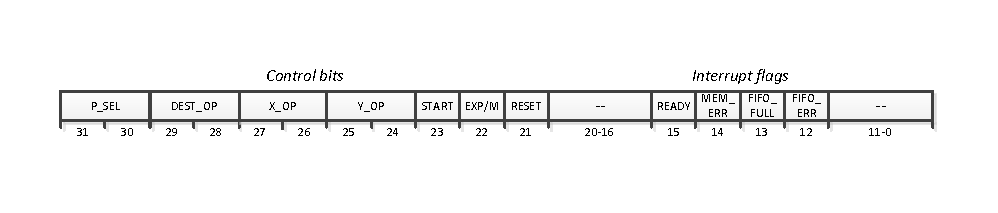
\includegraphics[trim=1.2cm 1.2cm 1.2cm 1.2cm, width=15cm]{pictures/axi_control_reg.pdf}
\caption{control register}
\end{figure}

\begin{tabular}{ll}
bits 31-30 	& P\_SEL : selects which pipeline part to be active\\
 			& $\bullet$  "01" lower pipeline part\\
 			& $\bullet$  "10" higher pipeline part\\
 			& $\bullet$  "11" full pipeline\\
 			& $\bullet$  "00" invalid selection\\
 			&\\
bits 29-28 	& DEST\_OP : selects the operand (0-3) to store the result in for a single\\
 			& Montgomery multiplication\footnotemark\\
 			&\\
bits 27-26 	& X\_OP : selects the x operand (0-3) for a single Montgomery multiplication\footnotemark[\value{footnote}]\\
			&\\
bits 25-24 	& Y\_OP : selects the y operand (0-3) for a single Montgomery multiplication\footnotemark[\value{footnote}]\\
			&\\
bit 23 		& START : starts the multiplication/exponentiation\\
			&\\
bit 22 		& EXP/M : selects the operating mode\\
 			& $\bullet$  "0" single Montgomery multiplications\\
 			& $\bullet$  "1" simultaneous exponentiations\\
 			&\\
bit 21		& unimplemented\\
			&\\
bit 20 		& RESET : active high reset for the core\footnotemark[2]\\
			&\\		
bits 19-16	& unimplemented\\
			&\\
bit 15		& READY : ready flag, "1" when multiplication is done\\
			& must be cleared in software\\
			&\\
bit 14		& MEM\_ERR : memory collision error flag, "1" when write error occurred\\
			& must be cleared in software\\
			&\\
bit 13		& FIFO\_FULL : FIFO full error flag, "1" when FIFO is full\\
			& must be cleared in software\\
			&\\
bit 12		& FIFO\_ERR : FIFO write/push error flag, "1" when push error occurred\\
			& must be cleared in software\\
			&\\
bits 11-0	& unimplemented\\
			&\\
\end{tabular}
\newline
\newline
\footnotetext[1]{when the core is running in exponentiation mode, the parameters DEST\_OP, X\_OP and Y\_OP have no effect.}
\footnotetext[2]{The reset affects the full IP core, thus resetting the control register, interrupt controller,
the multiplier pipeline, FIFO and control logic of the core.}
\newpage
\section{Interfacing the core's RAM}
Special attention must be taken when writing data to the operands and modulus. The least significant bit of the data has be on the lowest
address and the most significant bit on the highest address. A write to the RAM has to happen 1 word at a time, byte writes are not
supported due to the structure of the RAM.

\section{Handling interrupts}
When the embedded processor receives an interrupt signal from this core, it is up to the controlling software to
determine the source of the interrupt by reading out the interrupt flag of the control register.